\documentclass[a4paper,12pt]{article}

\usepackage{cmap}
\usepackage{mathtext}
\usepackage[T2A]{fontenc}
\usepackage[utf8]{inputenc}
\usepackage[english,russian]{babel}
\usepackage{indentfirst}
\usepackage{hyperref}
\frenchspacing


\usepackage{amsmath,amsfonts,amssymb,amsthm,mathtools} % AMS
\usepackage{icomma}

\DeclareMathOperator{\sgn}{\mathop{sgn}}

\newcommand*{\hm}[1]{#1\nobreak\discretionary{}
{\hbox{$\mathsurround=0pt #1$}}{}}

\usepackage{graphicx}
\graphicspath{{images/}{images2/}}
\setlength\fboxsep{3pt}
\setlength\fboxrule{1pt}
\usepackage{wrapfig}

\usepackage{array,tabularx,tabulary,booktabs}
\usepackage{longtable}
\usepackage{multirow}

\theoremstyle{plain}
\newtheorem{theorem}{Теорема}[section]
\newtheorem{proposition}[theorem]{Утверждение}
 
\theoremstyle{definition}
\newtheorem{corollary}{Следствие}[theorem]
\newtheorem{problem}{Задача}[section]
 
\theoremstyle{remark}
\newtheorem*{nonum}{Решение}

\usepackage{etoolbox}


\usepackage{extsizes}
\usepackage{geometry}
	\geometry{top=25mm}
	\geometry{bottom=35mm}
	\geometry{left=35mm}
	\geometry{right=20mm}

\usepackage{setspace}

\usepackage{lastpage}

\usepackage{soul}

\usepackage{hyperref}
\usepackage[usenames,dvipsnames,svgnames,table,rgb]{xcolor}
\hypersetup{
    unicode=true,
    pdftitle={Заголовок},
    pdfauthor={Автор},
    pdfsubject={Тема},
    pdfcreator={Создатель},
    pdfproducer={Производитель},
    pdfkeywords={keyword1} {key2} {key3},
    colorlinks=true,
    linkcolor=red,
    citecolor=black,
    filecolor=magenta,
    urlcolor=cyan
}

\usepackage{csquotes} % Еще инструменты для ссылок

%\usepackage[style=authoryear,maxcitenames=2,backend=biber,sorting=nty]{biblatex}

\usepackage{multicol} % Несколько колонок

\usepackage{tikz} % Работа с графикой
\usepackage{pgfplots}
\usepackage{pgfplotstable}

%\author{}
%\title{}
%\date{}

\begin{document} % конец преамбулы, начало документа
\subsection*{\begin{center}
Тест 2
\end{center}}
\begin{center}
\textbf{A.}
\end{center}
\fbox{
\begin{minipage}[c]{\textwidth}
\begin{description}
\item[1.]
На множестве $\mathbb{R}$ определено отношение $R$:
$(x, y) \in R$, если $x^3 - x = y^3 - y$.
\begin{description}
\item[(a)] Проверьте, что $R$ является отношением 
эквивалентности.
\begin{itemize}
\item рефлексивность $xRx$: $x^3 - x = x^3 - x$. $\checkmark$
\item симметричность $xRy \Rightarrow yRx$:
$x^3 - x = y^3 - y \; \Rightarrow \; y^3 - y = x^3 - x$. $\checkmark$
\item транзитивность $xRy \wedge yRz \Rightarrow xRz$: \\
$x^3 - x = y^3 - y \; \wedge \; y^3 - y = z^3 - z 
\; \Rightarrow \; x^3 - x = z^3 - z$. $\checkmark$
\end{itemize}
\item[(b)] Определите класс эквивалентности $[1]$.\\
\begin{scriptsize}
Классом эквивалентности $[a]\subset X$ 
элемента $a \in X$ называется подмножество элементов, 
эквивалентных $a$; то есть, 
\[
[a]=\{\,x\in X\mid x \sim a\,\}.
\] 
\end{scriptsize}
\[
[1] = \{ x \in \mathbb{R} | x^3 - x = 1^3 -1 = 0\} =
\{ -1, 0, 1\}.
\]
\end{description}
\item[2.]
Нарисуйте или обоснуйте, почему не существует
непересекающийся(планарный) граф с $5$ вершинами,
степени всех вершин которого равны $d(v) = 2$.\\
\begin{center}
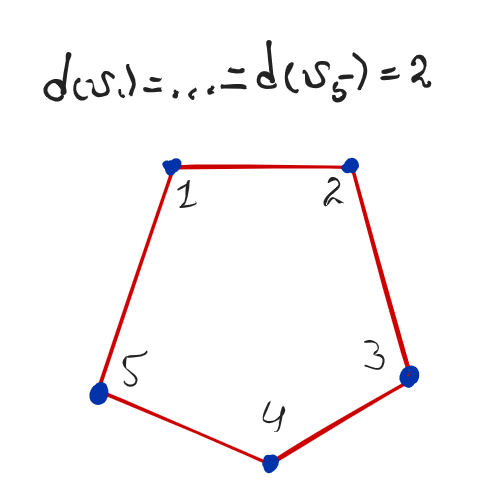
\includegraphics[scale=0.3]{2022-12-12_10-58.png}
\end{center}
\item[3.] Пусть у нас есть двудольный граф
$G = (V, E)$, $V = A \cup B$, $|A| = |B| =n$.
\begin{scriptsize}
Двудольный граф -- это граф, множество вершин которого 
можно разбить на две части таким образом, 
что каждое ребро графа соединяет вершину из одной части 
с какой-то вершиной другой части, 
то есть не существует рёбер между вершинами одной 
и той же части графа.
\end{scriptsize}
\begin{description}
\item[(a)] Каково максимально возможное число рёбер, 
которые может иметь граф $G$?\\
\[
n^2.
\]
\item[(b)] Каково минимально возможное число рёбер, которые
может иметь граф $G$?
\[
n.
\]
\end{description}
\end{description}
\end{minipage}
}
\begin{center}
\textbf{B.}
\end{center}
\fbox{
\begin{minipage}[c]{\textwidth}
\begin{description}
\item[1.] На множестве $\mathbb{N}$
задано отношение $R$: $(m, n) \in R$, 
если $|m - n| \leq 2$.
\begin{description}
\item[(a)] Выясните, является ли $R$ отношением эквивалентности.
\begin{itemize}
\item рефлексивность $mRm$: $|m-m| \leq 2$. $\checkmark$
\item симметричность $mRn \Rightarrow nRm$:
$|m - n| \leq 2 \; \Rightarrow \; |n - m| \leq 2$. $\checkmark$
\item транзитивность $mRn \wedge nRk \Rightarrow mRk$: \\
$|m - n| \leq 2 \; \wedge \; |n - k| \leq 2 
\; \nRightarrow \; |m - k| \leq 2$. \fbox{$\times$} \\
В качестве контпримера можно взять $m=0, n=2, k=4$.
\end{itemize}
\item[(b)] Определите все $n \in \mathbb{N}$,
для которых $(1, n) \in R \, \circ \, R$.
\[
\underbrace{|1-m| \leq 2}_{m = \{1, 2, 3\}}
 \; \wedge \; \underbrace{|m-n| \leq 2}_{m-2 \leq n \leq 2 + m}
 \quad \Longrightarrow \quad
 n = \{ 1, 2 , 3, 4, 5 \}
\]
\end{description}
\item[2.] Существует ли простой граф с $5$
вершинами и суммой степеней всех вершин $22$.
Если да, нарисуйте его. В противном случае обоснуйте ответ. \\
Нет, сумма степеней графа на $n$ вершинах не может быть
больше суммы степеней полного графа на $n$ вершинах $K_n$.
В нашем случае в $K_5$ $\sum d(v) = 5*4 = 20$, а по условию
задачи сумма степеней равна $22$, чего быть не может. 
\item[3.] Пусть у нас есть полный граф $K_n$: 
с вершинами $V = \{ 1, 2, \ldots , n \}$.
Сколько смежных подграфов графа $K_n$ имеют ровно два ребра?
\[
C^3_n
\]
\end{description}
\end{minipage}}
\begin{center}
\newpage
\textbf{C.}
\end{center}
\fbox{
\begin{minipage}[c]{\textwidth}
\begin{description}
\item[1.] На потенциальном множестве
$\mathcal{P}(\mathbb{N})$ мы имеем отношение $R$:
$(A, B) \in R$, если $A \subset B \cup \{ 1 \}$.
\begin{description}
\item[(a)] Определите, является ли $R$ рефлексивным
или транзитивным.
\begin{itemize}
\item рефлексивность $ARA$: $A \subset A \cup \{ 1 \}$. 
$\checkmark$
\item транзитивность $ARB \wedge BRC \Rightarrow ARC$: \\
$A \subset B \cup \{ 1 \} \; \wedge \; 
B \subset C \cup \{ 1 \}
\; \Rightarrow \; A \subset C \cup \{ 1 \}$. $\checkmark$
\end{itemize}
\item[(b)] Положим $B = \{ 2, 4 \}$.
Сколько множеств $A$ удовлетворяет $(B, A) \in R^{-1}$?
\[
b R^{-1} a \Leftrightarrow a R b
\] 
\[
A \subset \overbrace{\underbrace{B}_{\{2, 4\}} \cup \{ 1 \}}^{
\{ 1, 2, 4 \}} \quad \Longrightarrow \quad
A = \mathcal{P}(\{ 1, 2, 4\})
\]
\end{description}
\item[2.] Нарисуйте или обоснуйте, почему не существует
непересекающийся граф с $6$ вершинами, в котором
степени всех вершин равны $d(v) = 3$. \\
Это граф $K_{3, 3}$, который не является планарным.\\
\href{https://inlnk.ru/Pm9wRp}{См. док-во}
\item[3.] Пусть у нас есть полный граф $K_n$
с вершинами $V = \{ 1, 2, \ldots , n \}$.
Сколько путей длины $3$ ведёт между вершинами $1$ и $4$?
\[
(n-2) \cdot (n-3)
\]
\end{description}
\end{minipage}}
\begin{center}
\textbf{D.}
\end{center}
\fbox{
\begin{minipage}[c]{\textwidth}
\begin{description}
\item[1.]
На множестве $\mathbb{N}$ рассмотрим отношение $R$,
определённое следующем образом:
$(m , n) \in R$, $m \cdot n^4$ -- нечётное число.
\begin{description}
\item[(a)]
Определите, является ли $R$ рефлексивным или
симметричным.\\
$m$ и $n$ должны быть нечётными числами
\begin{itemize}
\item рефлексивность $mRm$: $m \cdot m^4$ - нечет. $\checkmark$
\item симметричность $mRn \Rightarrow nRm$:
$m \cdot n^4 - \text{нечет} \; \Rightarrow \; n \cdot m^4 - \text{нечет}$. $\checkmark$
\end{itemize}
\item[(b)] Выясните, какие числа $n \in \mathbb{N}$ 
удовлетворяют $(n, 1) \in R^{-1}$.
\[
\{ n | n = 2k +1 \, \wedge \, k \in \mathbb{Z}^{+} \}
\]
\end{description}
\item[2.] Нарисуйте или объясните, 
почему не существует простого графа с шестью вершинами,
для которого справедливо: 
две вершины имеют степень $d = 0$, 
две вершины имеют степень $d = 2$, 
и две другие вершины имеют степени $d \notin \{1, 2\}$.\\
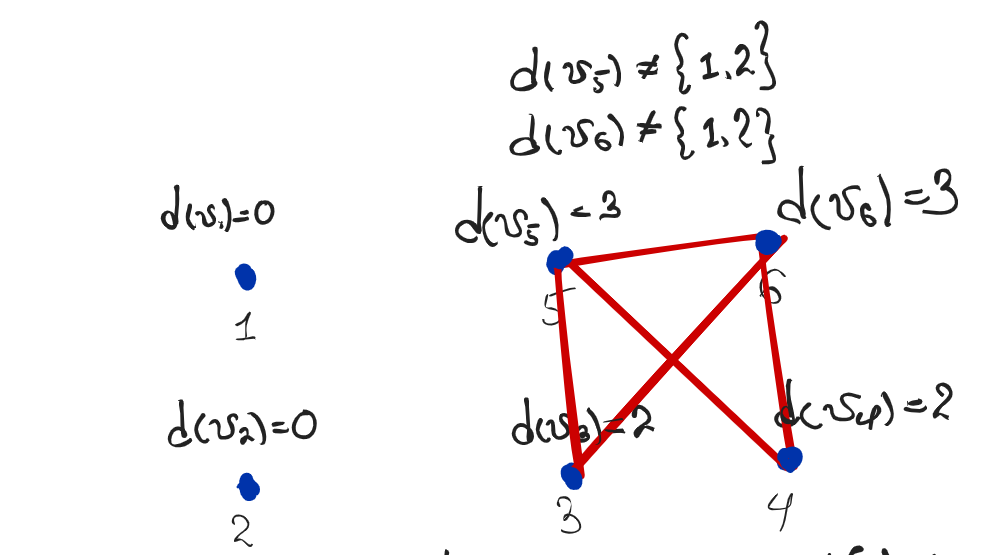
\includegraphics[scale=0.3]{2022-12-12_12-54.png}
\item[3.]  Пусть у нас есть полный граф 
$K_n$ с вершинами 
$V = \{1, 2, \ldots, n\}$. 
Сколько подграфов графа $K_n$, имеющих максимум одно ребро?
\[
C^2_n
\]
\end{description}
\end{minipage}}
\end{document} % конец документа





